\section{Technology Stack Roles Distribution} 
Before starting to explore the parts of Manolia 5.0 architecture in details and
analyzing how they solve the problems stated in \ref{thesis_problems} it is
important to clarify the communication relationships between the frameworks used
in the project. We also need to define which framework acts on the server-side
and which - on the client-side. Let us consider the high-level outline of
project's structure displayed on the figure \ref{fig:architecture}:

\begin{figure}[H] \centering 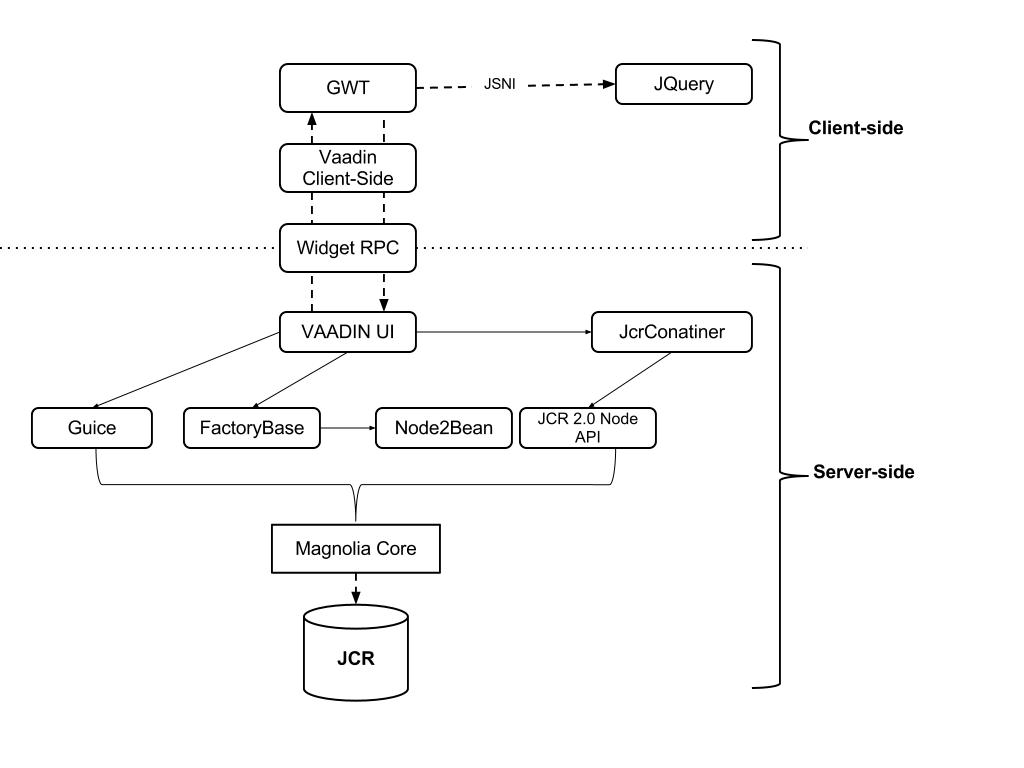
\includegraphics[width=\textwidth]{architecture.jpg}
	\caption{Magnolia CMS 5.0 Architecture}
	\label{fig:architecture}
\end{figure}

\paragraph{JCR} repository is at the lowest level of the hierarchy and stores
not only the content and templates but also all the configuration for the
system:
\begin{itemize}
  \item The structure of the user interface building blocks.
  \item Registries of the functionality units used within the system and the way
  they are accessible for the user.
  \item Binding between the action definitions that can be performed on the
  nodes and their implementation.
\end{itemize}

\paragraph{Magnolia Core} API's provide the low-level communication mechanism of
interaction with JCR and implementation for the various patterns that can be
re-used in the project. The most important parts of it include for instance the
API for querying the JCR and Node2Bean that allows for projecting the nodes to
Java Beans transparently to the developer. Another crucial framework provided by
the Magnolia Core is the Dependency Injection (DI) functionality based on Google Guice
\cite{google_guice}. The main strength of this framework is that allows to
define the mapping between the interface and the implementation of the
components right in a module descriptor - all the other configuration is done
internally and the developer does not have to take care of it, it is usually even
not necessary to know what DI mechanism actually provides the fucntionality.

\paragraph{Vaadin} layer is based on top of JCR and Magnolia Core API's. It
plays a role of the foundation for the AdminCentral web application. Vaadin
generates all the components and views of the system based on the information
provided by the configuraion. The datasources for the components are normally
provided in a form of the \texttt{JcrContainer} which is an implementation of
the Vaadin's \texttt{Conatiner} interface based on top of the JCR Node API.
Vaadin resides in the top level of the server-side architecture. 

\paragraph{Vaadin} interacts with the client-side by means of its core
communication mechanism (UIDL, see \ref{chapter_tech_stack}) and by means of an
additional API provided by the WidgetRPC add-on. The latter is used in order to
improve the clearness and simplicity of communication. UIDL
communication allows for passing the numerous variables between the client and
the server, resulting in rather complex code structures that analyse the
incoming changes.

Contrary to the plain UIDL, WidgetRPC allows for building the communication
interfaces and mutually call the methods between the component's counterpart,
making the conversation between them more fine-grained and roust.

Vaadin client-side part is responsible for handling both ways if the
communication and also controls the resuting UI presentation.

\paragraph{Finally, GWT} is responsible to produce the views on top the commands
and instructions that are coming through the Vaadin's client-side engine.
Whereas the simpliest vaadin applicaton does not require the programmer to engage
GWT into the development (core Vaadin's widgetset could be enough) Magnolia 5.0
project requires a variety of the custom components to be built so that the
resulting interface gets all the necessary components without significant
overhead caused by adopting the ones from the core. In order to increase the
performance and to provide some complex UI effects the JQuery library was
incorporated into the project's client-side ramework. The access to JQuery can
be done directly from GWT.
